\chapter{Background Physics	}

\section{Classical Chaos}
The concept of time evolution is one of the fundamental challenges in physics, how does a non-equilibrium state evolve over time? Even classically this problem can be challenging to approach. Chaos is typically defined such that a system is chaotic if its trajectory shows a significant dependence on its initial state. This causes its projection to be extremely weak to even small perturbations especially at longer times. \\
There exists however a set of systems which show non chaotic dynamics, these are known as integrable systems. \cite{dalessio_chaos}

\section{The Ergodic Hypothesis}
The first concept relevant to QMBS is the idea of ergodicity, the idea that underpins the idea of thermalization in microscopic systems. Ergodicity introduces the concept that a large enough sample of individual measurements can represent the bulk average of the entire system. 
The ergodic hypothesis, originally conjectured by Boltzmann as a method to link the microscopic dynamics with the ensemble average, implies that given long enough time, any non-equilibrium initial state will fully explore the entire phase space available from that initial state with the amount of time spent there being proportional to its volume. \\
\section{Thermalization}
Thermalization or Quantum Ergodicity is a quantum analogue to the classical ergodicity described above, wherein a many body system is separated into two subsystems one of which acts as a thermal sink which either disperses or absorbs energy to or from the other subsection such that it is possible to tend towards the thermal value as predicted by the statistical mechanics of the microcanonical ensemble. There are however examples of systems which are non ergodic, these systems have interesting non thermal dynamics even at long times. Understanding how these non-ergodic systems are produced and their dynamics is a growingly large field of research, there are a number of methods known as ergodicity breaking which describe different potential causes for the lack of ergodicity in a given quantum system are described below. These systems are of particular interest as these systems which avoid thermalization allow for quantum information encoded into the initial parameters to exist at long times. 
\subsection{Eigenstate Thermalization Hypothesis}
One of the key ideas within quantum many-body scaring is the idea that certain initial states can delay the process known as thermalization as is predicted by the Eigenstate Thermalization Hypothesis (ETH)\citep{srednicki_chaos_1994}. This phenomena is what allows for the periodic revivals as have been both experimentally and theoretically. The eigenstate thermalization hypothesis states that individual eigenstates of quantum ergodic systems act as thermal ensembles, therefore the systems long term dynamics are not defined by the initial conditions of the system. if we take a generic state $\ket{\Psi(0)} = \Sigma_a A_a \ket{a}$ where $\ket{a}$ is a many-body eigenstate of the system the time evolution of the state is described purely by the initial probabilities of finding the system in a given eigenstate, $P_a = |A_a|^2$.
\begin{equation}
  \ket{\Psi (t)} = e ^{-i\hat{H}t}\ket{\Psi(0)} = \Sigma_a A_ae^{-iE_nt}\ket{a}
\end{equation}  
The expectation value of an operator for a specific time T is given by $\expval*{\hat{O}} = \expval*{\hat{O}}{\Psi(T)}$ and we would expect the infinite time limit of this to approach the values predicted by the microcanonical ensemble
\begin{equation}
\expval*{\hat{O}}_\infty
= \lim_{T\rightarrow \infty} \frac{1}{T} \int_0^\infty \expval*{\hat{O}}{\Psi(T)} \dd t = \Sigma_a |A_a|^2\expval*{\hat{O}}{a}
\end{equation}
Since the infinite time value should be independent of the initial conditions it is reasonable to enforce that $\expval*{\hat{O}}{a}$ agrees with the canonical average since $|A_a|^2$ is dependent on $\ket{\Psi(0)}$. \citep{Abanin2019}
\\
The ETH also has significant implications on the entanglement of a many body system, 

\section{Ergodicity Breaking}
\subsection{Strong Ergodicity Breaking}
There are two different forms of ergodicity breaking, these are split into strong and weak ergodicity breaking. We define strong ergodicity breaking with the requirements that all eigenstates are non-ergodic, that is that the system never thermalizes.
\subsection{Weak Ergodicity Breaking}
The weak ergodicity breaking on the other hand requires for the system to almost always thermalize, that is there exists a small subset of eigenstates which fail to thermalize. 
\section{Quantum Many Body Scars}

\subsection{PXP Model}
The PXP model which is commonly used in QMBS experiments is based upon the idea of the Rydberg blockade and has experimentally shown non thermalizing dynamics \cite{bernien_probing_2017}.  The experiment consists of a system of two level atoms described by the states $\ket{\circ}$ and $\ket{\bullet}$ representing the ground and excited states. These states are allowed to flip freely when acted on by a microwave field via Rabi Oscillation. $\ket{\circ} \leftrightarrow \ket{\bullet}$. However when these Rydberg atoms are positioned close enough together the van der Walls forces repel. This distance can be tuned such that the interaction is strong enough to ensure that there are no two adjacent sites excited at the same time, $\ket{...\bullet \bullet ...}$. This is known as a Rydberg Blockade, a kinetic constraint on the system.

This model is effectively represented by the Hamiltonian 
\begin{equation}
\hat{H} = \sum_i P_{i-1}X_iP_{i+1}
\end{equation}

Where $X_i$ is the Pauli X gate $\sigma^x_i = \ket{\circ}_i\bra{\bullet}_i+\ket{\bullet}_i\bra{\circ}_i$, and $P_i$ acts as a projector onto the groundstate $P_i = \ket{\circ}_i\bra{\circ}_i$. Hence the name PXP. These projectors enforce the rydberg blockade constraint on the system.  

This constrained model has an interesting Hilbert Space. if we consider the simplest case with only two sites only the following sites are allowed $\ket{\circ \circ},\ket{\circ \bullet},\ket{\bullet \circ}$ since the $\ket{\bullet \bullet}$ is in violation of the Rydberg Blockade. From this it is apparent that the Hilbert Space cannot be represented as a tensor product state of the two separate Hilbert Spaces.
The majority of states in the PXP model thermalize rapidly, however there are a handful of states that fail to thermalize, one of such states is the N\'eel state or $\mathbb{Z}_2 = \ket{1010101...}$. \cite{turner_quantum_2018-1, chen_dynamics_2022}

\subsection{XY Heisenberg model} \label{sec:xymodel}

Recently QMBS were discovered experimentally in a 2D array of superconducting qubits \citep{zhang_many-body_2022}, wherein an approximate Su-Schreiffver-Heeger (SSH) model \cite{su_solitons_1979} constructed by alternating the coupling strengths between pairs of qubits. Experimentally a chain of pairs of qubits was produced within a 6x6 lattice of superconducting qubits. These pairs of qubits form 'dimers' where the intra-dimer coupling $J_a$ is larger than the inter-dimer $J_e$ coupling between them. If the system is constructed such that $J_a$ is significantly larger than $J_e$ and the system is half filled, that is when there are $L/2$ photons, where $L$ is the length of the chain, then each dimer acts as an independent two level system with one photon per dimer. The control of the photons in this model shows similarities to how electrons transfer through the polyacetylene in the SSH model. \\

Experimentally this model also has to consider the cross couplings between the qubits, the chosen physical layout of the dimers introduces a cross coupling term $J_x$, this cross coupling breaks the inegrability of the system and should allow the system to thermalize.

This system uses an XY model where finely tuned microwave pulses force rotations in the X and Y directions. This system shows different scarred states to the PXP model, in this model the states $\ket{\Pi}=\ket{D_+D_-D_+D_-...}$, $\ket{\Pi '}=\ket{D_-D_+D_-D_+...}$, where $\ket{D_-} = \ket{01}$ and $ \ket{D_+}=\ket{10}$ are found to have the non thermalizing dynamics expected of a QMBS. 

This system is an effective spin 1/2 XY model with the following effective hamiltonian. 
\begin{equation} \label{eq:eff_hamiltonian}
\mathcal{H}_{eff} /\hbar \approx \sum_{<i,j>}J_{ij} (S^+_iS^-_j + S^-_iS^+_j) +\sum_i \Omega_i S^+_iS_i^-
\end{equation}
where $J_{ij}$ is the effective coupling strength and $\Omega_i$ is the transition frequency which are both defined by the system design and coupling ratios. 


\subsubsection{SSH model}

The Su-Schriefer-Heeger model is based on the electron transfer in a polyacetaylene molecule \citep{su_solitons_1979}. The SSH model is one of the simplest examples of non trivial 1D topological chains. The SSH model shown in figure  \ref{fig:fig_SSH} was the influence of the alternating couplings in an attempt to partially decouple the subspaces within the superconducting XY model \citep{zhang_many-body_2022}, where they found QMBS phenomena within the subspace.

\begin{figure}
	\centering
	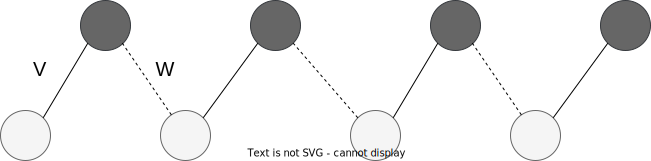
\includegraphics[width=0.5\linewidth]{SSH.png}
	\caption{Simple graphical representation of the SSH model, with alternating bond strengths. This is a representation of the repeating chain of double and single carbon-carbon bonds found in a molecule of polyacetylene.}
	\label{fig:fig_SSH}
\end{figure}

\section{Entanglement}

\subsection{Quantum Fisher Information}